\section{Results}
\label{sec:results}

\paragraph{Scheduling around life pays.} At a headline reserve of
$f_{\min}=\FminHead$ --- the ecosystem keeps 30\% of its daily light --- the
flat policy retains \FlatRetHead\% of the ecosystem-blind harvest value, while
the optimal temporal schedule retains \OptRetHead\%. That is a
\TemporalGainHead\% gain in harvested value at \emph{identical} ecological
cost, obtained purely by choosing \emph{when} to yield light to the biome
(Figure~\ref{fig:sweep}). The gain grows with the reserve: the more light the
ecosystem needs, the more a smart schedule matters, reaching
\TemporalGainMax\% at $f_{\min}=\TemporalGainMaxF$.

\begin{figure}[t]
\centering
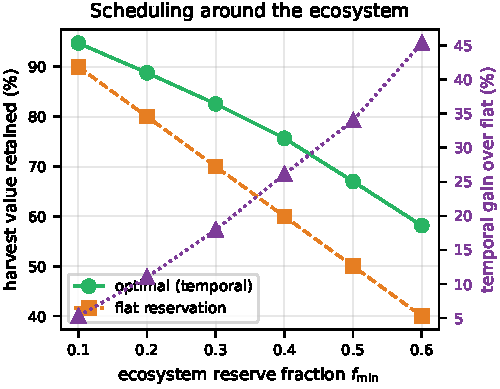
\includegraphics[width=0.85\linewidth]{figures/optimize_sweep.pdf}
\caption{Harvest value retained vs the ecosystem reserve fraction $f_{\min}$,
for the optimal temporal schedule and the flat reservation (both protect the
ecosystem equally). The temporal gain (right axis) widens as the reserve grows.}
\label{fig:sweep}
\end{figure}

\paragraph{What the schedule looks like.} Figure~\ref{fig:heatmap} shows the
optimal harvest fraction across bands and hours at $f_{\min}=\FminHead$,
overlaid with the demand curve. The schedule yields light to the ecosystem
around midday --- when supply is abundant and marginal harvest value is low ---
and harvests aggressively during the morning and evening demand peaks. This is
the concrete answer to the motivating question: an ecosystem that needs, say,
30\% of its daily light can be given that light in the hours we least want it,
leaving the valuable hours for harvesting.

\begin{figure}[t]
\centering
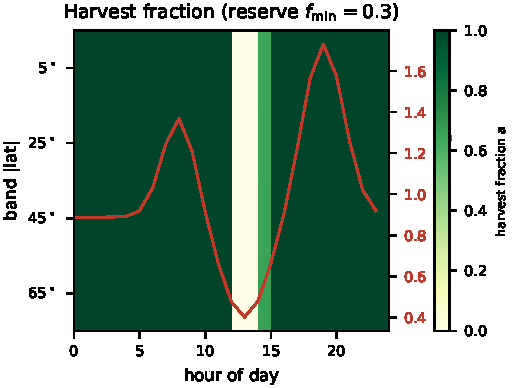
\includegraphics[width=0.85\linewidth]{figures/harvest_heatmap.pdf}
\caption{Optimal harvest fraction $a$ (green = harvest, pale = reserved for the
ecosystem) by latitude band and hour at $f_{\min}=\FminHead$, with the demand
weight (red). Light is yielded to the biosphere at low-value midday hours.}
\label{fig:heatmap}
\end{figure}

\paragraph{Putting the numbers together.} The picture is consistent across all
four questions. The Sun offers \InterceptedTW~TW; the surface receives
$\SurfaceGHI~\mathrm{W/m^2}$ on average; a conservative desert-and-rooftop
footprint already exceeds electricity demand \TimesElec-fold; orbit multiplies
per-collector power \SbspRatio$\times$ but chiefly by buying capacity factor;
and once we accept that surface light belongs to the biosphere, the way to
harvest more is not more area but better timing --- worth up to
\TemporalGainMax\% here. The bottleneck was never the Sun.
